\documentclass[12pt,a4paper]{article}
\usepackage{cmap}
\usepackage{amsmath}
\usepackage{mathtext}
\usepackage{titlesec}

\usepackage{minted} 

\usepackage[utf8]{inputenc}
\usepackage[T2A]{fontenc}
\usepackage{wrapfig}
\usepackage[english, russian]{babel}
\usepackage[left=2cm,right=2cm,top=2cm,bottom=2cm]{geometry}
\usepackage{indentfirst}

\DeclareSymbolFont{T2Aletters}{T2A}{cmr}{m}{it}

%%% Работа с картинками
\usepackage{graphicx}  % Для вставки рисунков
\graphicspath{{imgs/}}  % папки с картинками

\usepackage{caption}
\captionsetup{labelsep=period, labelfont=bf}

\titleformat{\section}[block]
{\normalfont}{\thesection.}{0 cm}{}

\titleformat{\subsection}[block]
{\bfseries}{\thesubsection.}{0 cm}{}

\titleformat{\subsubsection}[block]
{\bfseries}{\thesubsubsection.}{0 cm}{}

\titlespacing{\section}{17pt}{14pt}{10pt}
\titlespacing{\subsection}{17pt}{14pt}{4pt}
\titlespacing{\subsubsection}{17pt}{14pt}{4pt}

\def \TITLE {Отчет о выполнении лабораторной работы по информатике}
\def \SUBTITLE {Алгоритмы сортировки}
\def \AUTHOR {Выполнил студент группы Б03-405\\ Тимохин Даниил}
\def \DATE {11 сентября 2024 г.}

\begin{document}

\begin{titlepage}
	\centering
	\vspace{5cm}
	{\scshape\large Московский физико-технический институт \\
	(НАЦИОНАЛЬНЫЙ ИССЛЕДОВАТЕЛЬСКИЙ УНИВЕРСИТЕТ)}
	
	\vspace{4cm}
	{\LARGE \TITLE}
	
	\vspace{1cm}
	{\Huge\bf \SUBTITLE }
	
	\vspace{1cm}
	\vfill
	
\begin{flushright}
	{\LARGE \AUTHOR}
\end{flushright}
	

	\vfill

	\DATE
\end{titlepage}

\newpage

\fontsize{12}{14}\selectfont



\section{ Аннотация}
В работе изучается асимптотика различных алгоритмов сортировки и их зависимость от различных факторов. Реализация различных алгоритмов, замер их скорости.

\section{ Теоритические сведенья}
\subsection{ Измерение времени работы}
Для измерения времени работы кода используется функция
\begin{minted}{c++}
std::chrono::duration<double> timer(void (*my_sort)(int*, int, bool(int*,int*)), 
      int* array, int len, bool (*comp)(int*,int*)=&default_comp)
{
    auto start = std::chrono::high_resolution_clock::now();
    my_sort(array, len,comp);
    auto end = std::chrono::high_resolution_clock::now();
    if (test_result(array, len))
        return (end-start);
    else
        return std::chrono::duration<double>::zero();
}
\end{minted}


\subsection{ Тестирование}
Для записи результатов используется слдующий код, который несколько раз

\begin{minted}{c++}
for (int srt=0;srt<n_sorts;srt++)
    {
        for (unsigned long  p=1;p<=points;p++){
            for (int k=0;k<k_tests;k++)
            {
                len=(limits[srt]*p)/points;
                for (unsigned long  i=0;i<len;i++) array[i]=
                               rand_uns(INT16_MIN,INT16_MAX);
                //sort[srt](array,len,&default_comp);
                file<<names[srt]<<','<<len<<','<<
                      timer(sort[srt],array,len).count()<<'\n';
                file.flush();
                //if (test_result(array,len)) 
                //else continue;
            }
            std::flush(std::cout);
            std::cout<<'\r'<<"                                     "
                         <<'\r'<<names[srt]<<" "<<p/(points+.0)*100<<'%';
        }
        std::cout<<std::endl;
    }
\end{minted}

\newpage
\subsection{ Долгие сортировки}

\subsubsection{ Сортировка пузырьком}
\begin{minted}{c++}
void buble_sort(int* array, int len, bool (*comp)(int*,int*)=&default_comp)
{
    bool is_ready=true;
    for (int k=1;k<len;k++)
    {
        is_ready=true;
        for (int i=0;i<len-k;i++)
            if (!comp(array+i,array+i+1))
            {
                swap((array+i),(array+i+1)); 
                is_ready=false;
            }
        if (is_ready) break;
    }
}
\end{minted}

\subsubsection{ Сортировка выбором}
\begin{minted}{c++}
void choose_sort(int* array, int len, bool (*comp)(int*,int*)=&default_comp)
{
    for (int i=0;i<len;i++)
        for (int j=i+1;j<len;j++)
            if (!comp(array+i,array+j))
                swap(array+i,array+j);
}
\end{minted}

\subsubsection{ Сортировка Шейкером}
\begin{minted}{c++}
void shaker_sort(int* array, int len, bool (*comp)(int*,int*)=&default_comp)
{
    bool is_ready=true;
    int l=0,r=len-1,i=0;
    while (r-l>0)
    {
        for (;i<r;i++)
            if (!comp(array+i,array+i+1))
                {
                    swap(array+i,array+i+1);
                    is_ready=false;
                }
        r--;
        for (;i>l;i--)
            if (!comp(array+i-1,array+i))
                {
                    swap(array+i-1,array+i);
                    is_ready=false;
                }
        l++;
        if (is_ready) break;
    }
}
\end{minted}

\subsubsection{ Сортировка вставкой}
\begin{minted}{c++}
void put_sort(int* array, int len, bool (*comp)(int*,int*)=&default_comp)
{
    int *p=new int;
    for (int i=1;i<len;i++)
    {
        *p=*(array+i);
        for (int j=0;j<i;j++)
            if (comp(p,array+j))
            {
                shift_data(array+j,i-j);
                swap(p,array+j);
                break;
            }
    }
    delete p;
}
\end{minted}

\subsection{ Быстрые сортировки}
\subsubsection{ Сортировка расчёской}
\begin{minted}{c++} 
void comb_sort(int* array, int len, bool (*comp)(int*,int*)=&default_comp)
{
    int d=len/1.25;
    bool is_ready=true;
    while (d>1)
    {
        for (int i=0;i<len-d;i++)
            if (!comp(array+i,array+i+d))
            {
                swap((array+i),(array+i+d));
            }
        d/=1.25;
    }
    d=1;
    while (true)
    {
        is_ready=true;
        for (int i=0;i<len-1;i++)
            if (!comp(array+i,array+i+1))
            {
                swap((array+i),(array+i+1));
                is_ready=false;
            }
        if (is_ready) break;
    }
}
\end{minted}

\newpage
\subsubsection{ Сортировка слиянием}
\begin{minted}{c++}
void merge_sort(int* array, int len, bool (*comp)(int*,int*)=&default_comp)
{
    int* array_dop = new int[len];
    int d=1,i,j,st,k;
    while (d<len)
    {
        for (st=0;st<len;st+=2*d)
        {
            i=st;
            j=st+d;
            for (k=0;k<2*d;k++)
            {
                if (i==st+d || j==st+2*d || j>=len || i>=len) break;
                if (comp(array+i,array+j))
                    *(array_dop+st+k)=*(array+i++);
                else
                    *(array_dop+st+k)=*(array+j++);
            }
            for (; i < len && i<st+d; i++)
            {
                *(array_dop+st+k)=*(array+i);
                k++;
            }
            for (; j < len && j<st+d*2; j++)
            {
                *(array_dop+st+k)=*(array+j);
                k++;
            }
        }
        d<<=1;
        std::memcpy(array,array_dop,len*sizeof(int));
    }
    delete [] array_dop;
}
\end{minted}

\newpage
\subsubsection{ Быстрая сортировка}
\begin{minted}{c++}
void quick_sort(int* array_s,int start, int len,
        bool (*comp)(int*,int*), int* array_dop_s, int leni) 
{
    if (len<2) return;
    int* array=array_s+start;
    int* array_dop=array_dop_s+start;
    if (len==2)
    {
        if(!comp(array,array+1)) swap(array,array+1);
        return;
    }
    int l=0,r=len-1;
    int* op=array+len/2;
    for (int k=0;k<len;k++)
    {
        if (k==len/2) continue;
        if (comp(array+k,op))
        {
            *(array_dop+l)=*(array+k);
            l++;
        }
        else
        {
            *(array_dop+r)=*(array+k);
            r--;
        }
    }
    *(array_dop+l)=*op;
    std::memcpy(array,array_dop,((unsigned long long)len)*sizeof(int));
    quick_sort(array_s,start, l, comp, array_dop_s, leni);
    quick_sort(array_s,start+l+1, len-(l+1), comp, array_dop_s, leni);
}

void quick_sort(int* array, int len, bool (*comp)(int*,int*)=&default_comp)
{
    int* array_dop=new int[len];;
    quick_sort(array,0,len,comp,array_dop,len);
    delete [] array_dop;
}
\end{minted}

\newpage
\subsubsection{ Сортировка кучей}
\begin{minted}{c++}
void heap_sort(int* array, int len, bool (*comp)(int*,int*)=&default_comp)
{
    heap(array,len,comp);    
    for (int i=len;i>1;i--)
    {
        update_heap(array,i,comp);
        swap(array,array+i-1);
    }
}

void update_heap(int* array, int len, bool (*comp)(int*,int*)=&default_comp, 
int head=0,bool reverse=false)
{
    if (head>len) return;
    bool a=false,b=false;
    if (head*2+1<len)
        if (comp(array+head,array+head*2+1) ^ reverse){a=true;}
    if (head*2+2<len)
        if (comp(array+head,array+head*2+2) ^ reverse){b=true;}
    if (a==b && a==true)
    {
            if (comp(array+head*2+2,array+head*2+1) ^ reverse)
            {
                swap(array+head,array+head*2+1);
                update_heap(array,len,comp,head*2+1);
            }
            else
            {
                swap(array+head,array+head*2+2);
                update_heap(array,len,comp,head*2+2);
            }
            return;
    }
    if (a)
    {
        swap(array+head,array+head*2+1);
        update_heap(array,len,comp,head*2+1);
    }
    if (b)
    {
        swap(array+head,array+head*2+2);
        update_heap(array,len,comp,head*2+2);
    }
    
}

void heap(int* array, int len, bool (*comp)(int*,int*)=&default_comp,
int head=0,bool reverse=false)
{
    for (int i = len / 2 - 1; i >= 0; i--) update_heap(array, len, comp, i);
}
\end{minted}

\newpage
\section{ Оборудование}
{\bfseries Intel Core i5-7300HQ CPU @ 2.50GHz}

{\bfseries 8Гб оперативной памяти}

{\bfseries Немного свободного времени}

\section{ Результаты измерений и обработка данных}

\subsection{Общие результаты}
Проведём несколько тестов. Сначала построим все графики в одном маштабе.
\begin{figure}[!ht]
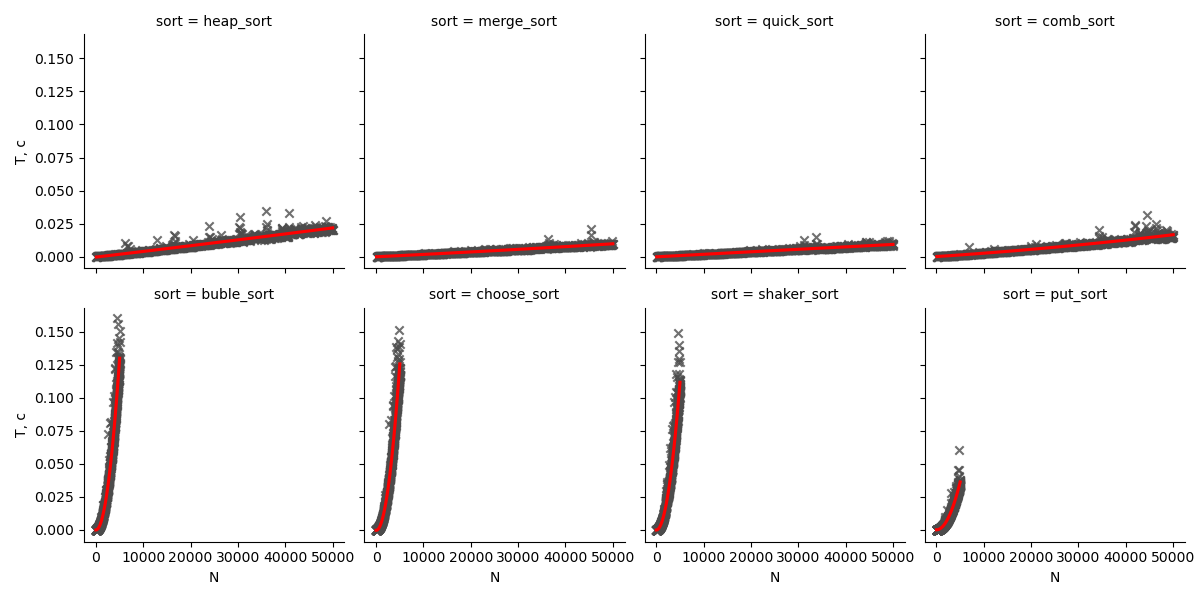
\includegraphics[width=\textwidth]{imgs/compare_all.png}
\caption{Зависимость времени выполнения от количества элементов}
\end{figure}

Мы видим, что первые четыре работают намного быстрее, чем "плохие сортировки". Поэтому проверим соответствуют ли "хорошие" зависимости $O(n\log n)$, а плохие $O(n^2)$.

\subsection{Доказательство асимптотик}
Построи мграфик для медленных сортировок в логарифмических координатах.
\begin{figure}[!ht]
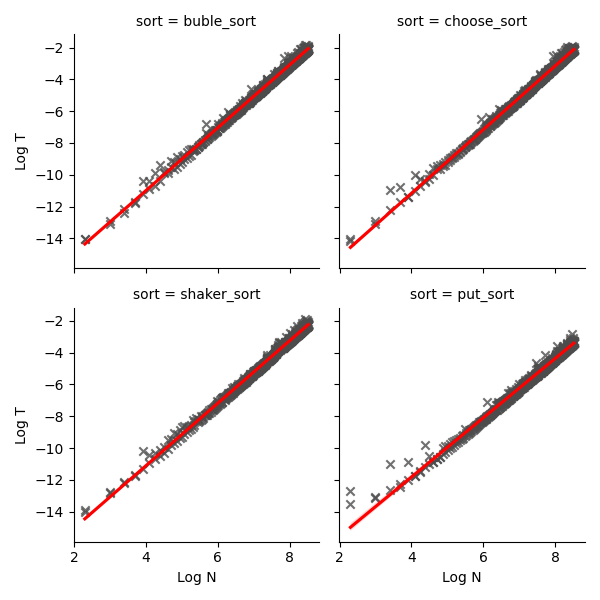
\includegraphics[width=\textwidth]{imgs/compare_n2.png}
\caption{Зависимость времени выполнения от количества элементов в логорифмическом маштабе}
\end{figure}
Мы видим, что на грфике все прямые имеют коэффицент наклона $\approx2$, а значит мы можем с уверенностью сказать, что их асимптотическая сложность по времени равна $O(n^2)$.

\clearpage
Теперь построим график зависимости $T/N$ от $\log N$ для "быстрых" сортировок.
\begin{figure}[!ht]
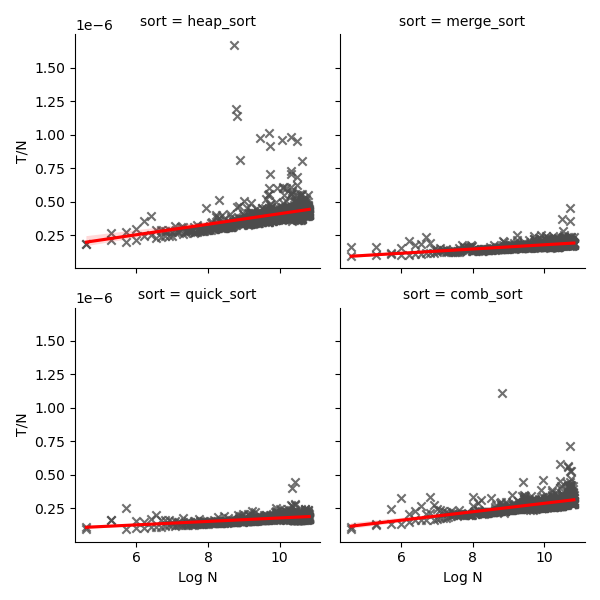
\includegraphics[width=\textwidth]{imgs/compare_log.png}
\caption{Зависимость времени выполнения от количества элементов для быстрой сортировки}
\end{figure}

Тут тоже видно, что асимптотика сортировок с высокой точностью соответствует $O(n \log n)$, так как мы видим прямые при аппроксимации.

\subsection{Немого про зависимость от данных}
Рассмотрим время выполнения сортировок от входных данных. Будем смотреть на отсортированные данные, отсортированные в обратном порядке и случайные данные.
\begin{figure}[!ht]
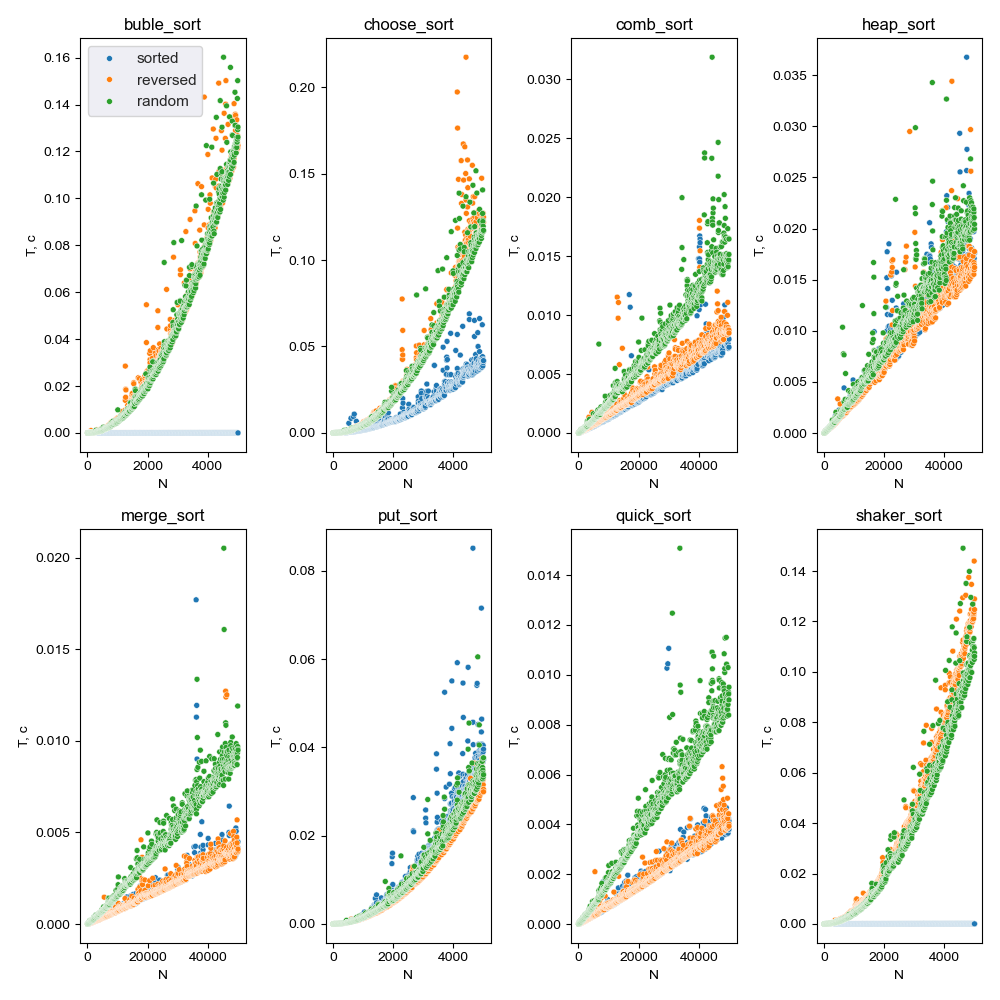
\includegraphics[width=\textwidth]{imgs/compare_by_data.png}
\caption{Зависимость времени выполнения от начальных данных}
\end{figure}

Видно, что для сортировки пузырьком и шйкера время для отсортированного массива почти 0. это из-за того, что мы сделали оптимизацию на остановку алгоритма при получении отсортированного массива. Остальные льшь получают приемущество в том, что на отсортированных или перевёрнутых данных можно пропускать действия и намного быстее выполнять операции. Это происходит за счёт предсказателя ветвлений. Так как все условия верны/неверны, то процессор может заранее начать обрабатывать инструкции из условия. На неупорядоченных данных это сложнее, так как мы е можем точно предсказать результат ветвления.

\subsection{Немого про зависимость от оптимизации компилятором}
Проведём тесты для четырёх вариантов оптимизации -O0, -O1, O2, -O3.
\begin{figure}[!ht]
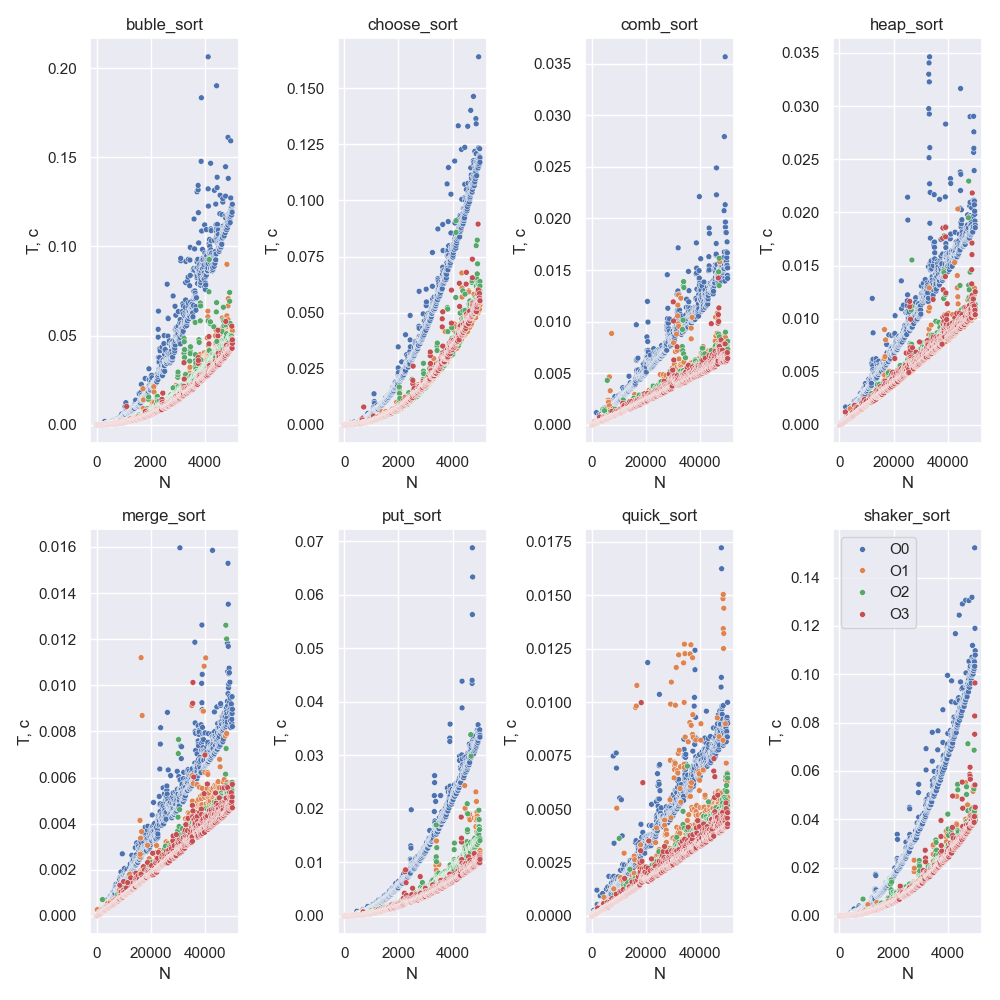
\includegraphics[width=\textwidth]{imgs/compare_by_optimizaion.png}
\caption{Зависимость времени выполнения от оптимизации}
\end{figure}
Заметим, что уже с -O1 дальнейшая оптимизация компилятором значительных приемуществ не даёт. Это проиходит так как при написании кода не было ориентации на использование определённых аппаратных ускорений, поэтому при компиляции сложнее найти участки кода, соответствующие стандартным случаям, которые можно заменить. Поэтому можно сделать вывод, что так как -O3 достаточно нестабильная сборка, то в стандартных задачах -O2 и -O1 могут покрыть все потребности. Выбор лишь зависит от времени, которое пользователь готов затратить на компиляцию.

\subsection{Небольшое исследование}
\begin{figure}[!ht]
\begin{tabular}{cc}
{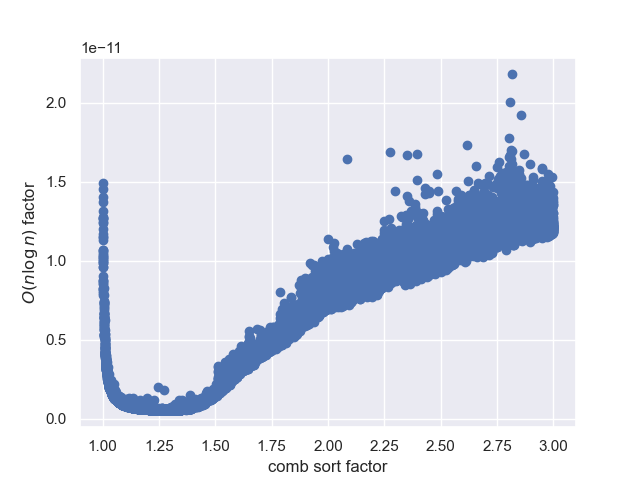
\includegraphics[width=0.45\textwidth]{imgs/comb_logn_fc.png}} &
{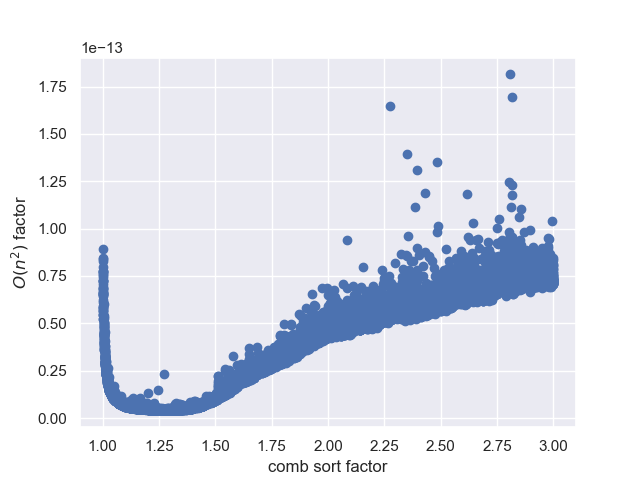
\includegraphics[width=0.45\textwidth]{comb_n2_fc.png}} \\
{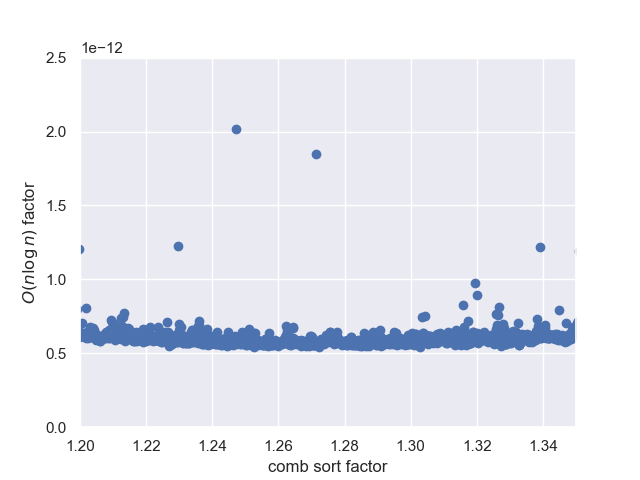
\includegraphics[width=0.45\textwidth]{imgs/comb_logn_fcsc.png}} &
{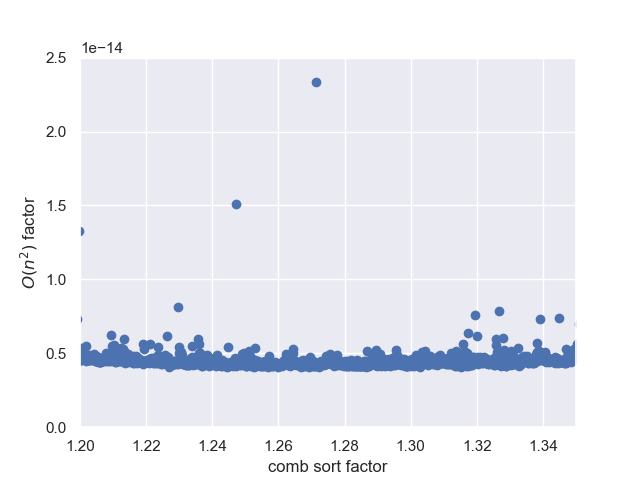
\includegraphics[width=0.45\textwidth]{comb_n2_fcsc.png}} 
\end{tabular}
\caption{Завиимость коэффициента для сложности от вактора в сортировке расчёской}
\end{figure}
Быо принято решение попробовать найти лучший фактор для сортировки расчёской. В ходе тестов получилось, что $factor \in (1.22; 1.34)$. В других случаях средняя сложность превращается в квадратичную. Разбро сдля квадрата меньше, чем для логорифма

\newpage
\subsection{Работа при малых числах}
Видно, что даже на малых $n$ эффективные алгоритмы лучше справляются со своей задачей, чем медленные.
\begin{figure}[!ht]
\begin{tabular}{c}
{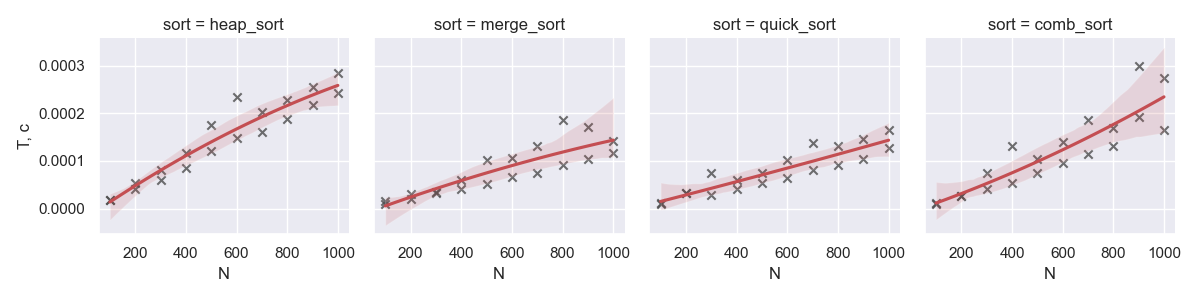
\includegraphics[width=\textwidth]{imgs/compare_all_sm1.png}}\\
{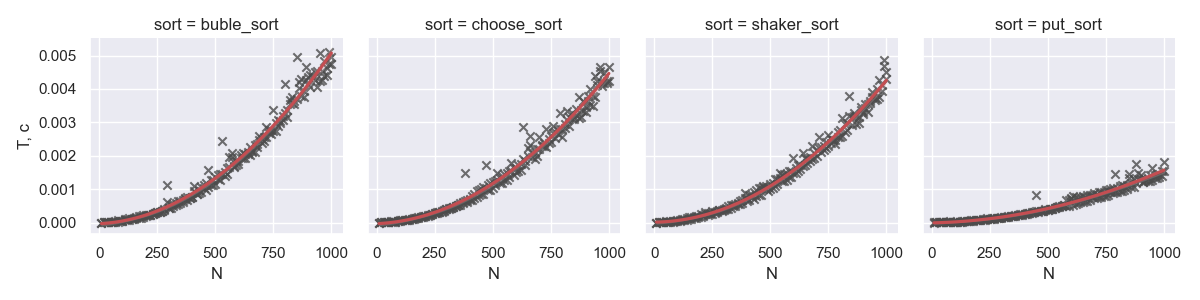
\includegraphics[width=\textwidth]{imgs/compare_all_sm2.png}}
\end{tabular}
\caption{Первый грфик, но с ограничением в 1000 элементов}
\end{figure}

\newpage
\section{Выводы}
В ходе работы были исследованы особенности сортировок, а также созданы собственные их реализации. Полученные данные говорят о явных превоходствах эффективных алгоритмов над квадротичными. Но при этом быстрые сортировки гораздо сложнее в реализации и есть большая вероятность допустить ошибку в указателях. Одной из самых эффективных среди медленных оказалась сортировка вставками. Скорее всего это происходит за счёт аппаратного ускорения сдвига. При этом наиболее быстрыми среди эффективных получились "быстрая" и сортировка слиянием, так как там используется большое количество достаточно предсказуемых ветвлений и действий.
\end{document}